%!TEX root=document.tex

\section{{\large \SeeDB} Front-End \& Architecture}
\label{sec:system_architecture}

%In this section, we present an overview of the \SeeDB\ architecture.
% Given an input query on a dataset, the goal of \SeeDB is to recommend
% visualizations the analyst would find most valuable.
% \SeeDB recommends visualizations that the analyst would find most valuable,
% taking into account aspects such as the background, user preferences,
% and context (as discussed in Section~\ref{sec:general-metric}).

We now describe \SeeDB's front-end user experience, and then
describe the architecture and the execution engine in more detail.

\stitle{Front-end Experience.} 
We packaged \SeeDB as a recommendation plugin that can
be incorporated into a visualization tool such as Tableau or Spotfire. 
For evaluating our system, we have combined \SeeDB with a simple visualization
builder interface inspired by Polaris~\cite{polaris}.
Figure~\ref{fig:frontend1} shows the web front-end for \SeeDB 
comprising four parts 
(A) dataset selector used to connect to a database and query a specific collection of tables; 
(B) query builder used to
formulate queries using a form-based interface; 
(C) visualization builder used to manually specify visualizations; and 
(D) \SeeDB recommendations plugin 
that displays recommended visualizations.
The recommendations provided by \SeeDB change in 
response to changes in the query (B)
issued against the database.
\resolved{\srm{This is the first mention of ``human in the loop'' philosophy.  I think it might be good
to promote this to an earlier part of the paper, but only if we feel like we have something interesting
to say about it.}}
%SRM cut this -- we already said it and it doesn't really matter to VLDB reviewers
%Note that supporting basic visualization specification 
%capabilities a la Polaris, coupled with automated recommendations enabling
%the reduction of tedious manual effort,
%implies that \SeeDB will form part of a
%{\em mixed initiative}~\cite{mixed_initiative} data exploration tool.

\resolved{delete rest, too detailed:
We note that the {\em mixed-initiative} design of \SeeDB incorporating both manual
visualization specification and automated recommendations, reflects the
human-in-the-loop philosophy underlying \SeeDB.
We seek to speed up the analytics process not by completely automating the task, but
by providing the analyst real-time support while letting him or her drive the process.
}

\begin{figure}[htb]
\vspace{-15pt}
\centerline{
\hbox{\resizebox{8cm}{!}{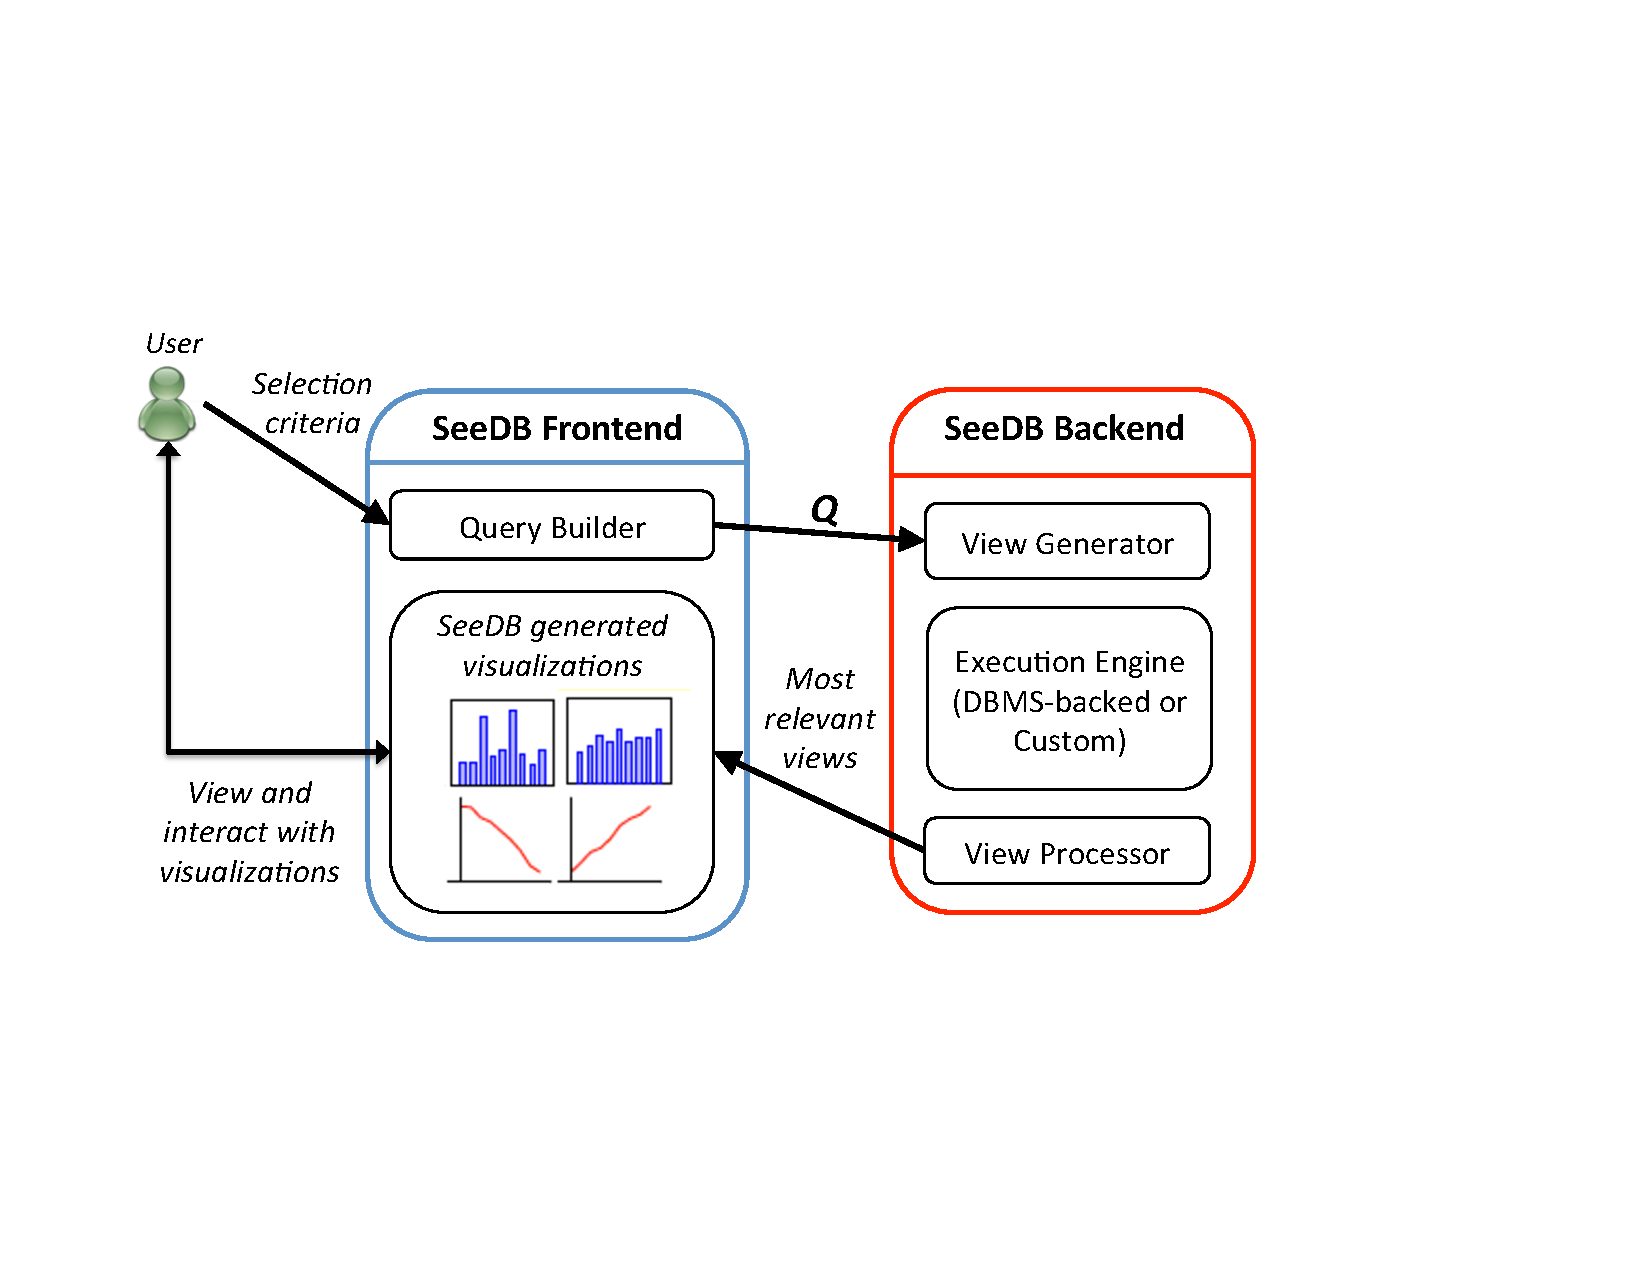
\includegraphics[trim=0 0 0 0, 
clip=true]{Images/seedb-architecture.pdf}}}}
\vspace{-12pt}
\caption{SeeDB Architecture}
\vspace{-10pt}
\label{fig:sys-arch}
\end{figure} 


\stitle{Architectural Overview.} 
\SeeDB is implemented as a middleware layer that can run on
top of any SQL-compliant database system. 
Figure \ref{fig:sys-arch} depicts the overall architecture of our
system.  The \SeeDB client is a web-based front-end that captures user
input and renders visualizations produced by the \SeeDB server.  The
\SeeDB server is composed of two main components. The first
component, the {\it view generator}, is responsible for parsing the
input query, querying system metadata and generating the list of
visualization queries that must be evaluated.  
The goal of the {\em execution engine} is to evaluate the collection of queries
 using our optimizations on top of
the underlying DBMS.
The selected aggregate views (i.e., those with high deviation) 
are sent to the \SeeDB client 
and are displayed as visualization recommendations to the user, 
who can then interact with these
visualizations.

\stitle{Basic Execution Engine.} 
To motivate the need for optimizations, we now describe 
how our execution engine would work if we had no optimizations. 
To identify the $k$ best aggregate views,
\SeeDB needs to do the following:
For each aggregate view, it generates
a SQL query corresponding to the target
and reference view, and issues
the two queries, one at a time, to the underlying DBMS.
It repeats this process for each aggregate view.
As the results are received, \SeeDB computes the
distance between the target and reference view
distributions, and identifies the $k$ visualizations
with highest utility. 

Naturally, this basic implementation has many inefficiencies.
In a table with $a$ dimensions, $m$ measures, and $f$ aggregation functions, 
$2\times f \times a \times  m$ queries must be executed independently.  
As we show in Section~\ref{sec:experiments}, this can take >100s for
large data sets (with hundreds of attributes and millions of rows).
These latencies are unacceptable for interactive use.

\stitle{Execution Engine with Optimizations.} 
To reduce latency in 
evaluating the collection of aggregate views, 
the execution engine  
applies two kinds of optimizations:
{\em sharing}, where aggregate view queries are combined to share computation
as much as possible, and {\em pruning}, where aggregate view queries
corresponding to low utility visualizations are dropped from consideration without scanning the whole
dataset.
These optimizations are largely orthogonal to each other.
To derive benefits from both these kinds of optimizations,
we develop a {\em phased execution framework}.
Each phase operates on a subset of the dataset.
Phase $i$ of $n$ operates on the $i$th of $n$ equally-sized partitions of the dataset. 
(Empirically, we have found $n=10$ to
work well, though our results are not very sensitive to the value
of $n$.) 
For instance, if we have $100,000$ records and $10$ phases,
the $i = 4$th phase processes records $30,001$ to $40,000$.
The execution engine begins 
with the entire set of aggregate views under consideration.
\begin{denselist}
\item During phase $i$, the execution engine updates the partial results
for the set of aggregate views
still under consideration using the $i$th fraction of the dataset.
The execution engine applies {\em sharing-based optimizations}
to minimize scans of the $i$th fraction of the dataset by combining
DBMS queries and executing them in tandem.
\item At the end of phase $i$, the execution engine uses 
{\em pruning-based optimizations} to determine which aggregate views to discard.
The partial results of each aggregate view on the fraction from $1$ through $i$ are used to 
estimate the quality of each view, and the views with low utility are discarded. 
\end{denselist}
The retained aggregate views are then processed on the $i+1$th round,
and the process continues. 
In this manner, the set of views under consideration
decreases across these phases, with all aggregate views at the start 
of the first phase, and only the $k$ views left
at the end of the $n$th phase.
%Further, in this manner, the sharing and pruning based optimizations do
%not interfere with each other---one is applied during the phase,
%and one is applied at the end of the phase.
\papertext{The pseudocode for the phase based execution framework
can be found in the extended technical report~\cite{seedb-tr}.}

We next describe the \SeeDB optimizations,
specifically, the sharing based optimizations in Section~\ref{sec:sharing_opt} and 
the pruning based optimizations in Section~\ref{sec:pruning_opt}.
\techreport{
\begin{algorithm}[h]
\caption{Pruning Framework}
\label{algo:custom_exec_engine}
\begin{algorithmic}[1]
\State viewsInRunning $\gets$ \{all views\}
\State currPhase $\gets$ 0
\While {currPhase.hasNext()}
\State processNextPartition()
%\State updateUtilityEstimates()
\If {currPhase.End()}
\State pruneViews(viewsInRunning)
\State currPhase.Next()
\EndIf
% \If {stoppingCondition.True()}
% \State break
% \EndIf
\EndWhile
\State return viewsInRunning.sort().getTopK()
\end{algorithmic}
\end{algorithm}
\agp{I've pasted this as is but needs to be updated.}
}
% \reviewer {
% 	D2.5 The horizontal partitioning is never detailed: how is it done? How is the
% number of fragments decided?
% }
% \mpv{something about how partitions are defined}




 
\begin{figure}[htb]
\centerline{
\hbox{\resizebox{9cm}{!}{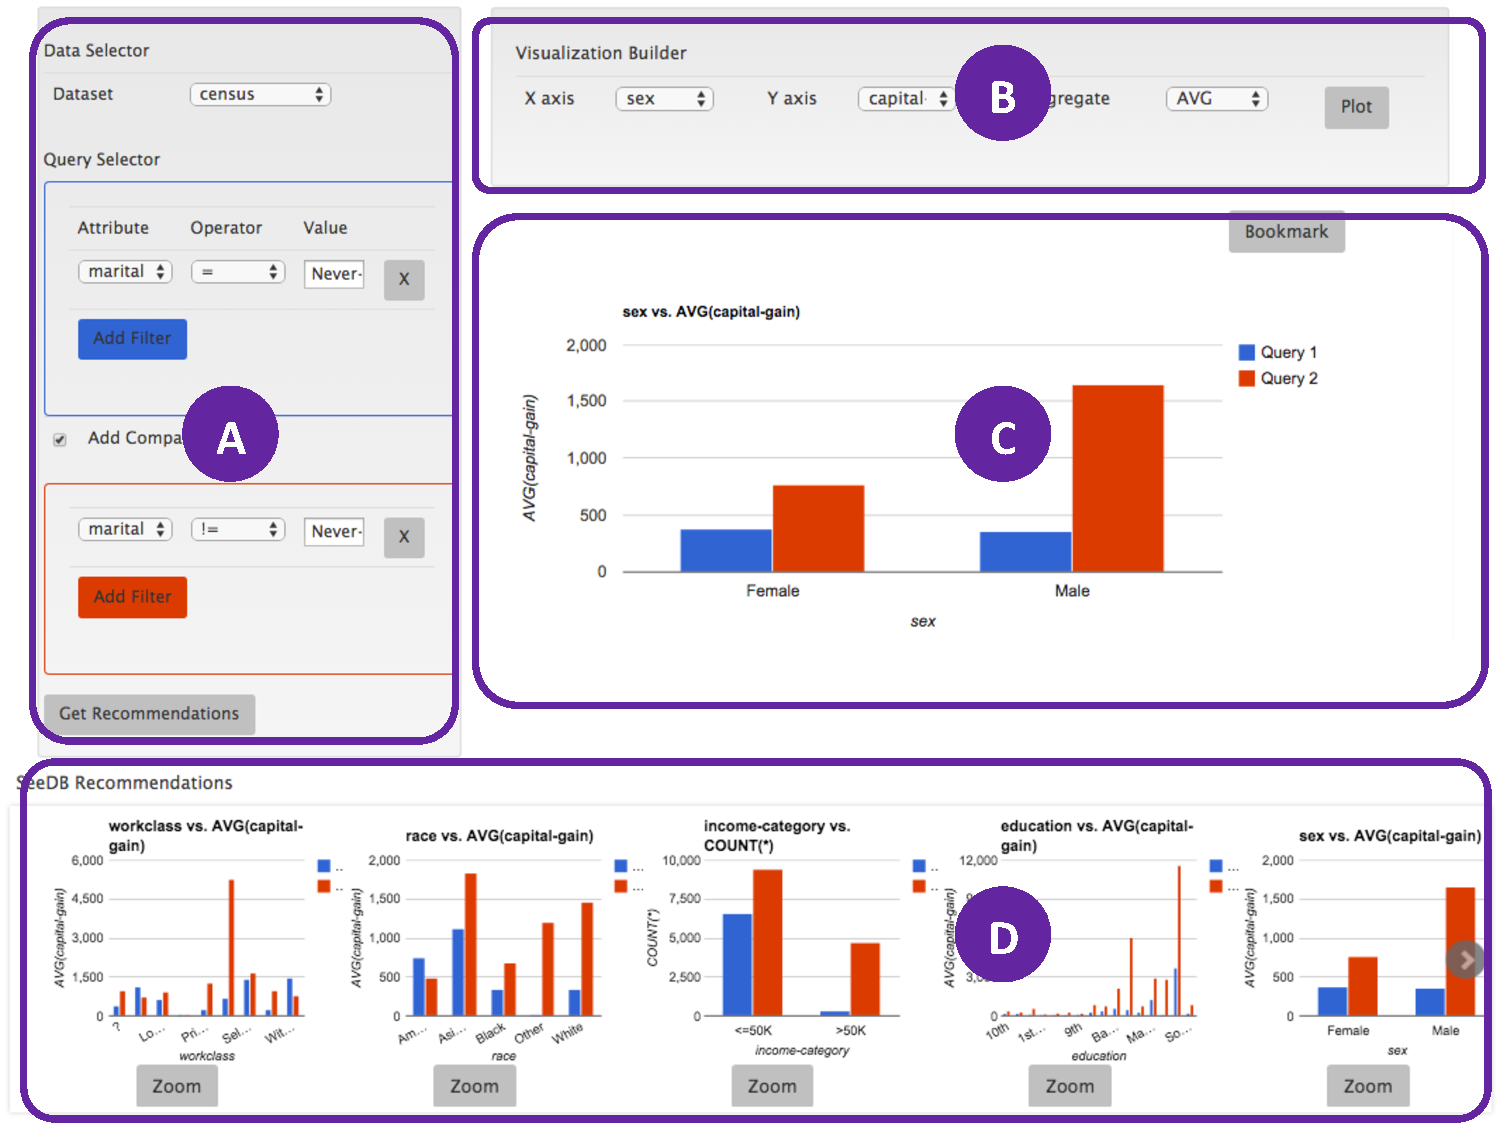
\includegraphics[trim=0mm 0mm 0mm 0mm,
clip=true]{Images/seedb_frontend.pdf}}}}
\caption{\SeeDB Frontend}
\vspace{-20pt}
\label{fig:frontend1}
\end{figure} 


% The optimizer applies multi-query
% optimization 
%  which is responsible for applying multi-query 
% optimization (Section \ref{}) to combine and rewrite DBMS queries 
% corresponding to view in running.
% Next, the execution engine issues optimized queries to the underlying DBMS
% and performs post-processing to compute results for individual views.
% Results from the execution engine are then fed to the pruner which leverages
% view pruning techniques to discard low-utility views.
% The set of views that pass muster with the pruner re-enter the optimizer for
% the next phase of execution.
% Once \SeeDB has identified the top views, the results are returned to the client 
% where \SeeDB frontend generates and displays the recommended visualizations.

% the view generator module queries the system metadata for table sizes, 
% column types, and correlations between column values. 
% It then uses this metadata and the incoming query to remove redundant aggregate views and generate ``stubs'' for the remaining aggregate views.
% The view stubs are then passed to the execution engine which is responsible 
% executing the aggregate views and performing run-time view pruning to identify
% high-utility views.
% To execute aggregate views, the execution engine optimizes the set of aggregate
% views, turns view stubs into SQL queries, and uses the underlying DBMS to efficiently execute the aggregate queries. \mpv{Fix sentence}.
% Once the \SeeDB server has executed the aggregate views and identified the top-k
% views, the data underlying top views is sent to the client where \SeeDB frontend 
% generates and displays the recommended visualizations.

% However, in this work, for ease of development and testing, we built 
% \SeeDB as a standalone end-to-end system that allows users to pose 
% arbitrary queries over data and obtain recommended visualizations.

% The standalone version of \SeeDB\ is comprised of two main components: 
% a light-weight client that is 
% used to issue queries, display recommended visualizations, and allow basic 
% interactions with visualizations; 
% and a server used to generate candidate
% aggregate views, execute
% them over data and identify the aggregate views with highest utility. 
% Figure \ref{fig:sys-arch} depicts the architecture of our system.
% Once the analyst chooses the data of interest (by issuing a query $Q$), the
% client makes a call to the backend for visualization recommendations for $Q$.
% Aggregate view stubs are essentially more elaborate triples of the form $(a, m, f)$ as discussed in Section \ref{sec:problem_statement}. 


% The generated aggregate view stubs are then sent to the execution engine
% responsible for querying the underlying data, evaluating the utility of each
% candidate view, and identifying the top views of interest. 

% Figure \ref{fig:frontend1} shows the \SeeDB client in action; including the supported mechanisms to specify an input query 
% and the visualizations generated by a sample query. 

% In the backend, the view generator module queries the system metadata for table sizes, 
% column types, and correlations between column values. 
% It then uses this metadata and the incoming query to remove redundant aggregate views and generate ``stubs'' for the remaining aggregate views. 
% Aggregate view stubs are essentially more elaborate triples of the form $(a, m, f)$ as
% discussed in Section \ref{sec:problem_statement}. 
% The generated aggregate view stubs are then sent to the execution engine
% responsible for querying the underlying data, evaluating the utility of each
% candidate view, and identifying the top views of interest. 
% Once the \SeeDB\ backend has identified the best aggregate views, the \SeeDB\
% client generates and displays recommended visualizations based on these views.
% Figure \ref{fig:frontend1} shows the \SeeDB client in action; including the supported mechanisms to specify an input query 
% and the visualizations generated by a sample query. 



% In this paper, we build the execution engine in three stages. 
% In the first stage \mpv{better word?}, we implement \SeeDB as a layer on top of the database system and apply traditional multi-query optimization 
% techniques to see how far we can push existing relational databases to support a \SeeDB-type workload.
% While we obtain resonable performance for small datasets, we find the optimizations are insufficient to support large datasets \mpv{quantify?}.
% Therefore, next, we develop a set of pruning techniques that can use running estimates of utility to rapidly prune low-utility views. 
% By reducing the number of views evaluated, these techniques reduce overall latency and also allow \SeeDB to return results without processing the entire dataset.
% We implement these pruning strategies in a simple shared scan system to test the efficacy of our techniques.
% Finally, we build a hybrid execution engine that combines our pruning strategies with the performance optimizations of the DBMS-backed execution engine,
% thus giving us the best of both worlds. 

% In this paper, we explore two distinct implementations of the \SeeDB\ execution
% engine. 
% Our first implementation draws upon traditional multi-query optimization~\cite{}
% and OLAP literature~\cite{} to implement \SeeDB\ as a wrapper
% on top of a database system. \mpv{These techniques are usually inside the DBMS, 
% we are using them outside?}
% The goal of this implementation is to study how far 

% While we obtain reasonable performance by employing well-known optimizations, we find that 
% operating through the SQL interface limits the performance we can obtain.
% Therefore, we next built a custom execution engine that completely shares query scans between
% all views and uses heuristics to rapidly prune low-utility views.
% These techniques allow us to perform only a single pass over the data
% and rapidly identify top visualizations. \mpv{Incorp into DB?}
% However, existing systems do not provide a good means to share scans between
% queries or to access intermediate results during scans.
% As a result, optimization opportunities are limited.
% To overcome the constraints of existing database systems, we implement a
% simple, custom Execution Engine for \SeeDB\ optimized to share scans
% across all views and perform pruning based on intermediate results. 
% In an ideal solution, shared scans and pruning would be implemented inside the
% database; however, for the purpose of this work, we implement the \SeeDB\
% execution engine as a standalone proof-of-concept with a brief discussion of how
% the \SeeDB\ engine could be made part of a DBMS. \mpv{need to add this discussion 
% somewhere}

% Next we briefly examine the \SeeDB client and then describe the execution engines
% in detail.

% In the DBMS-based execution engine (Section \ref{}), the view stubs are passed
% through the optimizer that identifies the best ways to combine the queries to minimize
% execution time.
% Once the views have been optimized, the views are rewritten as SQL queries and
% executed against the underlying database. 
% The results of these queries are
% processed to update the view stubs and compute view utility. 
% Once all the queries have been processed, the top-k views are returned to the
% frontend.
% 
% In the main-memory execution engine, \SeeDB\ makes a single pass through the
% data (either read from disk or already present in memory) and keeps running
% estimates of utility for each of the views stubs obtained from the View
% Generator. 
% As the engine processes more of the data, the utility estimates become more
% accurate and \SeeDB\ uses various pruning heuristics to prune out views on the fly.
% By the time the full data has been processed, \SeeDB\ has identified the top-k
% views with the largest utility that are then returned to the frontend.


